\documentclass[conf]{new-aiaa}
%\documentclass[journal]{new-aiaa} for journal papers
\usepackage[utf8]{inputenc}

\usepackage{graphicx}
\usepackage{amsmath}
\usepackage{commath}
\usepackage[version=4]{mhchem}
\usepackage{siunitx}
\usepackage{longtable,tabularx}
\usepackage{float}
\usepackage{listings}
\usepackage{color} %red, green, blue, yellow, cyan, magenta, black, white
\definecolor{mygreen}{RGB}{28,172,0} % color values Red, Green, Blue
\definecolor{mylilas}{RGB}{170,55,241}
\setlength\LTleft{0pt} 

\lstset{language=Matlab,%
	%basicstyle=\color{red},
	breaklines=true,%
	morekeywords={matlab2tikz},
	keywordstyle=\color{blue},%
	morekeywords=[2]{1}, keywordstyle=[2]{\color{black}},
	identifierstyle=\color{black},%
	stringstyle=\color{mylilas},
	commentstyle=\color{mygreen},%
	showstringspaces=false,%without this there will be a symbol in the places where there is a space
	numbers=left,%
	numberstyle={\tiny \color{black}},% size of the numbers
	numbersep=9pt, % this defines how far the numbers are from the text
	emph=[1]{for,end,break},emphstyle=[1]\color{red}, %some words to emphasise
	%emph=[2]{word1,word2}, emphstyle=[2]{style},    
}

% ================================================================ % 
\title{ASE 389P.4 Methods of Orbit Determination \\ Homework 1: Basic Orbit Propagation}

\author{Junette Hsin}
\affil{Masters Student, Aerospace Engineering and Engineering Mechanics, University of Texas, Austin, TX 78712}

\begin{document}

\maketitle

\begin{abstract}
This assignment is designed to provide a basic introduction on how to propagate an orbit. MATLAB was used to complete the assignment. 
\end{abstract}


% ================================================================ % 
\section{Introduction}

In this assignment, a tool was created to numerically propagate a circular orbit about the Earth and to convert between Cartesian and Keplerian orbital elements. The software implemented in this assignment will be used later in the course provides additional background and/or a review of basic orbital mechanics.



% ================================================================ % 
\section{Problem 1}

\subsection{Statement} 
\begin{center}
\fbox{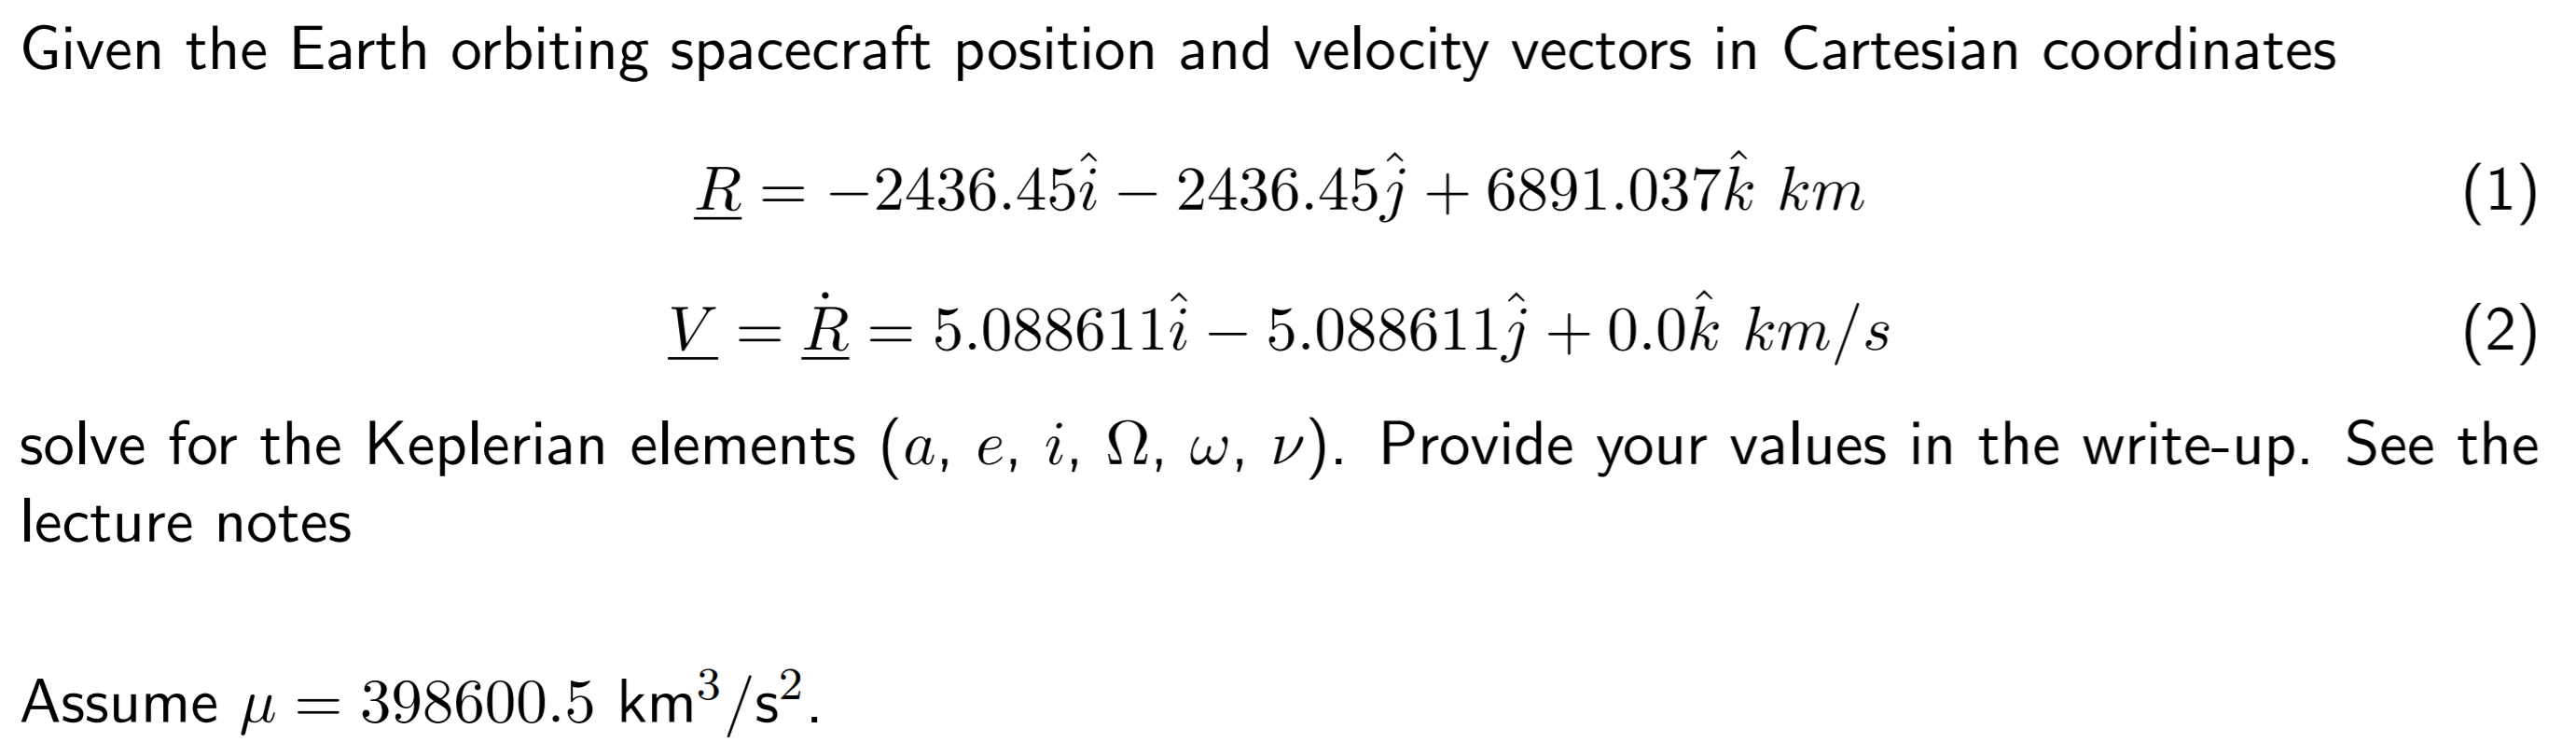
\includegraphics[width=0.9\textwidth]{prob_1.png}} \\
\end{center}

% -------------------------------- % 
\subsection{Solution} 

The algorithms to convert orbital elements to Cartesian and back were taken from Reference \cite{bate_astrodynamics}. Given the spacecraft position and velocity vectors from the problem statement, the Keplerian elements are: 

\begin{equation}
\begin{aligned}
a = &~ 7.712184983762814e+03 \\ 
e = &~ 0.447229247404423 \\ 
i = &~ 1.570796326794897 \\ 
\omega = &~ 3.139593866862924 \\ 
\Omega = &~ 3.926990816987241 \\ 
\nu = &~ 2.032461649676350  
\end{aligned}
\end{equation}

where $a$ is the semi-major axis, $e$ is the eccentricity, $i$ is the orbit inclination, $\omega$ is the argument of perigee, $\Omega$ is the right ascension of the ascending node, and $\nu$ is the true anomaly. 

% ================================================================ % 
\section{Problem 2} 

\subsection{Statement} 
\begin{center}
\fbox{
\includegraphics[width=0.9\textwidth]{prob_2.png}} \\
\end{center}

% -------------------------------- % 
\subsection{Solution} 



% ================================================================ % 
\section{Problem 3} 

\subsection{Statement} 
\begin{center}
	\fbox{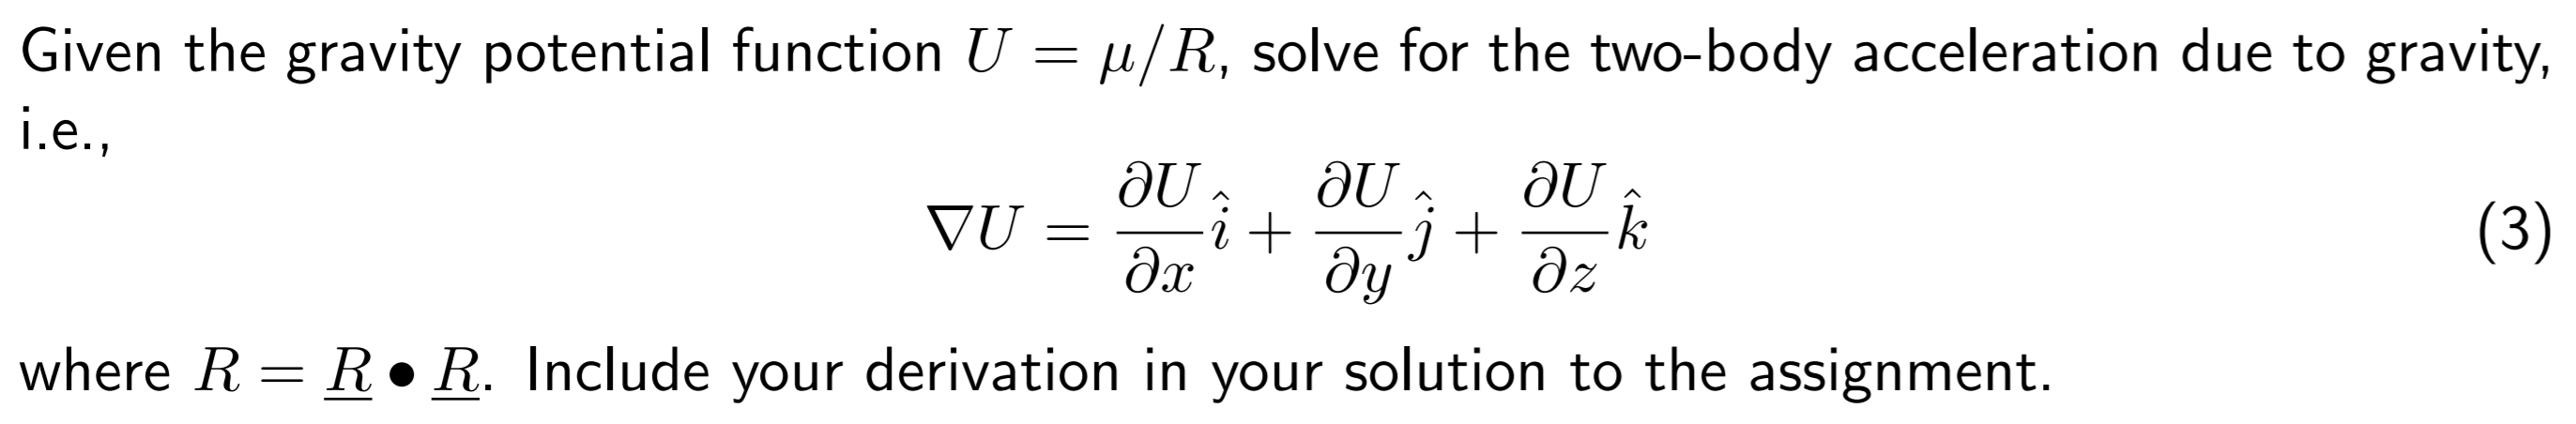
\includegraphics[width=0.9\textwidth]{prob_3.png}} \\
\end{center}

% -------------------------------- % 
\subsection{Solution 1} 

To solve for the two-body acceleration due to gravity, first calculate R, which is given in the problem statement as $R = \underline{R} \cdot \underline{R}$. Let us first define \underline{R} as the following: 

\begin{equation}
\underline{R} = x \hat{i} = y \hat{j} + z \hat{k}
\end{equation}

The dot product of the vector \underline{R} with itself is equal to the square of its magnitude: 

\begin{equation}
R = \underline{R} \cdot \underline{R} = x^2 + y^2 + z^2
\end{equation}

Given the gravity potential function $U = \mu/R$, the gradient of the gravity potential function $ \nabla U $ is:

\begin{equation}
\nabla U = \frac{\delta U}{\delta x} \hat{i} + \frac{\delta U}{\delta y} \hat{j} + \frac{\delta U}{\delta z} \hat{k}  
\end{equation} 

First derive $\dfrac{\delta U}{\delta x} \hat{i}$: 

\begin{equation}
\frac{\delta U}{\delta x} \hat{i} = \dfrac{\delta \Big( \dfrac{\mu}{R} \Big) }{\delta x} \hat{i} = \dfrac{ \delta \Big( \dfrac{\mu}{x^2 + y^2 + z^2} \Big) }{\delta x} \hat{i}
\end{equation}

Take the partial derivative: 

\begin{equation}
\dfrac{ \delta \Big( \dfrac{\mu}{x^2 + y^2 + z^2} \Big) }{\delta x} \hat{i} = \dfrac{ \delta \big(\mu ( x^2 + y^2 + z^2 )^{-1} \big) }{\delta x} \hat{i} = -\mu ( x^2 + y^2 + z^2 )^{-2} ( 2x ) \hat{i}
\end{equation}

Now simplify: 

\begin{equation}
-\mu ( x^2 + y^2 + z^2 )^{-2} ( 2x ) \hat{i} = -\dfrac{2 \mu x}{ (x^2 + y^2 + z^2 )^2 } \hat{i}
\end{equation}

Thus: 

\begin{equation}
\dfrac{\delta U}{\delta x} \hat{i} = -\dfrac{2 \mu x}{ (x^2 + y^2 + z^2 )^2 } \hat{i}
\end{equation}

$\dfrac{\delta U}{\delta y} \hat{j} $ and $\dfrac{\delta U}{\delta z} \hat{k} $ can be derived through the same process, which result in the following: 

\begin{equation}
\dfrac{\delta U}{\delta y} \hat{j} = -\dfrac{2 \mu y}{ (x^2 + y^2 + z^2 )^2 } \hat{j}
\end{equation}

\begin{equation}
\dfrac{\delta U}{\delta z} \hat{k} = -\dfrac{2 \mu z}{ (x^2 + y^2 + z^2 )^2 } \hat{k}
\end{equation}

The gradient of the gravity potential function is thus: 

\begin{equation}
\nabla U = -\dfrac{2 \mu x}{ (x^2 + y^2 + z^2 )^2 } \hat{i} -\dfrac{2 \mu y}{ (x^2 + y^2 + z^2 )^2 } \hat{j} -\dfrac{2 \mu z}{ (x^2 + y^2 + z^2 )^2 } \hat{k}
\label{eq:grad_U}
\end{equation}

Plug in $x = -2436.45$, $y = -2436.45$, $z = 6891.037$, and $\mu = 398600.5$ from Problem 1 into Equation \ref{eq:grad_U} to solve for the two-body acceleration due to gravity: 

\begin{equation}
\nabla U = 5.512551407304731e-07 \hat{i} - 5.512551407304731e-07 \hat{j} - -1.559120676071291e-06 \hat{k} 
\end{equation}

% -------------------------------- % 
\subsection{Solution 2}

The gravitational potential function is commonly simplified as $\nabla U = \mu/r$, where $r$ is the distance between two bodies \cite{bate_astrodynamics}. Therefore: 

\begin{equation}
r = \sqrt{R} = \sqrt{\underline{R} \cdot \underline{R}} = ( \underline{R} \cdot \underline{R} )^{1/2} = ( x^2 + y^2 + z^2 )^{1/2}
\label{eq:U_r}
\end{equation}

If we use Equation \ref{eq:U_r} to calculate the gradient for the potential function, then $\dfrac{\delta U}{\delta x} \hat{i}$ becomes: 

\begin{equation}
\frac{\delta U}{\delta x} \hat{i} = 
\dfrac{\delta \Big( \dfrac{\mu}{r} \Big) }{\delta x} \hat{i} = 
\dfrac{ \delta \Big( \dfrac{\mu}{ ( x^2 + y^2 + z^2 )^{1/2} } \Big) }{\delta x} \hat{i} = 
\dfrac{\delta \big( \mu ( x^2 + y^2 + z^2 )^{-1/2} \big) }{ \delta x }
\end{equation}

Take the derivative and simplify: 

\begin{equation}
\dfrac{\delta \big( \mu ( x^2 + y^2 + z^2 )^{-1/2} \big) }{ \delta x } = 
 \mu \Big( -\frac{1}{2} \Big) ( x^2 + y^2 + z^2 )^{-3/2} ( 2x ) \hat{i} = 
 - \dfrac{\mu x}{ ( x^2 + y^2 + z^2 )^{3/2} } \hat{i}
\end{equation}

Thus: 

\begin{equation}
\frac{\delta U}{\delta x} \hat{i} = - \dfrac{\mu x}{ ( x^2 + y^2 + z^2 )^{3/2} } \hat{i} = - \dfrac{\mu x}{r^3} \hat{i}
\end{equation}

And: 

\begin{equation}
\frac{\delta U}{\delta y} \hat{j} = - \dfrac{\mu y}{r^3} \hat{j}
\end{equation}

\begin{equation}
\frac{\delta U}{\delta z} \hat{k} = - \dfrac{\mu z}{r^3} \hat{k}
\end{equation}

Equation \ref{eq:grad_U} then becomes: 

\begin{equation}
\nabla U = - \dfrac{\mu x}{r^3} \hat{i} - \dfrac{\mu y}{r^3} \hat{j} - \dfrac{\mu z}{r^3} \hat{k}
\label{eq:grad_U_r}
\end{equation}

Plug in $x = -2436.45$, $y = -2436.45$, $z = 6891.037$, and $\mu = 398600.5$ from Problem 1 into Equation \ref{eq:grad_U_r} to solve for the two-body acceleration due to gravity: 

\begin{equation}
\nabla U = 0.002123566317530 \hat{i} + 0.002123566317530 \hat{j} - 0.006006104810708 \hat{k}
\end{equation}




% ================================================================ % 
\section{Problem 4} 

\subsection{Statement} 
\begin{center}
	\fbox{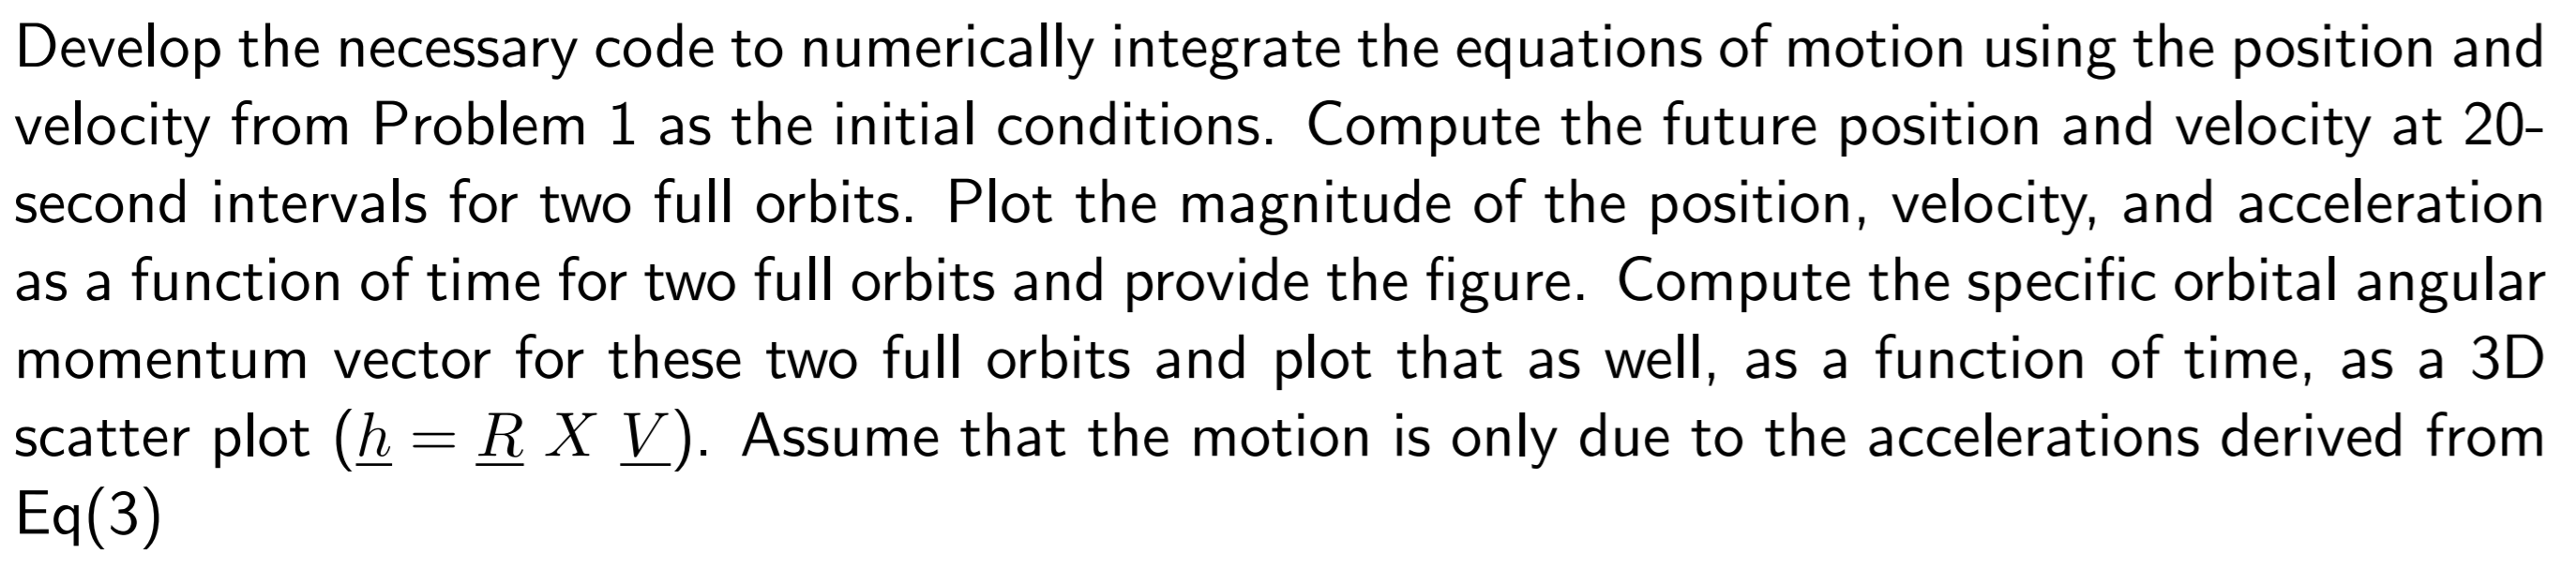
\includegraphics[width=0.9\textwidth]{prob_4.png}} \\
\end{center}

% -------------------------------- % 
\subsection{Solution} 

The period for the orbit was found by using the semi-major axis in the following equation: 

\begin{equation}
T   = \abs{2 \pi \sqrt{a^3 / \mu}}       % period 
\end{equation}

The orbit was propagated by numerically integrating the equations of motion \ref{eq:grad_U_r} for 2 periods using \texttt{ode45}. The relative and absolute tolerances were set to 1e-8. The acceleration was calculated by differentiating velocity with respect to time, and then the magnitudes of the position, velocity, and acceleration were plotted in Figure \ref{fig:prob4_2bodeom}. 

%toler   = 1e-8;         % 1e-14 accurate; 1e-6 coarse 
%options = odeset('reltol', toler, 'abstol', toler ); 
%[t,x] = ode45(@TwoBod_6states, [0 2*T], [r; v], options); 

\begin{figure}[H]
	\centering
	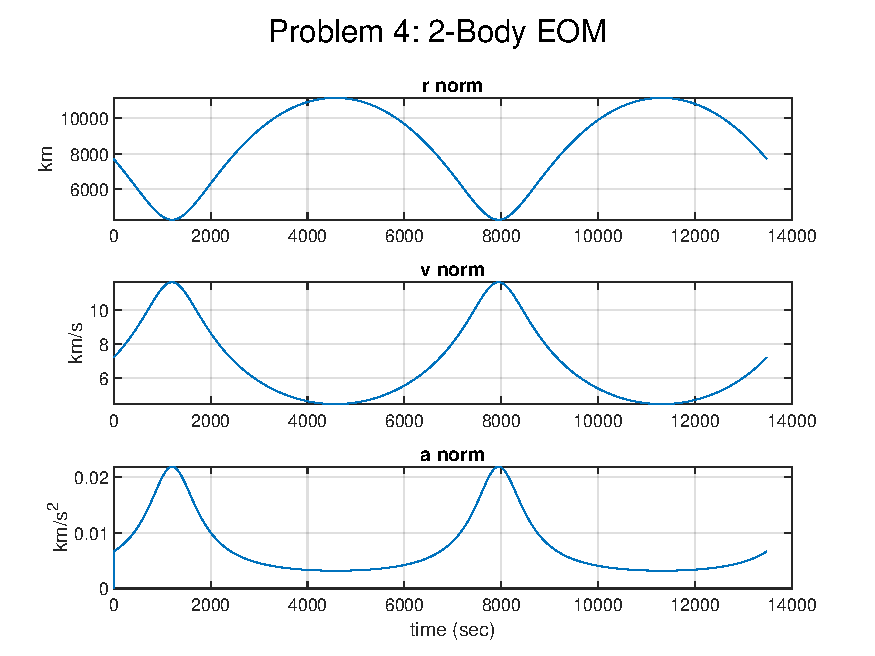
\includegraphics{prob4_2bodeom.pdf}
	\caption{}
	\label{fig:prob4_2bodeom}
\end{figure}

The magnitudes of the velocity and acceleration vary throughout the orbit, which indicates that the orbit is not circular. The position and velocity vectors were converted into orbital elements which are shown in \ref{fig:prob4_2bodoes}. All of the orbital elements with the exception of true anomaly remain essentially constant, revealing the predictable and Keplerian nature of the orbit. The eccentricity shows that the orbit is elliptical; an eccentricity of 0 forms a perfectly circular orbit and a 1 forms a parabolic escape orbit. 

\begin{figure}[H]
	\centering
	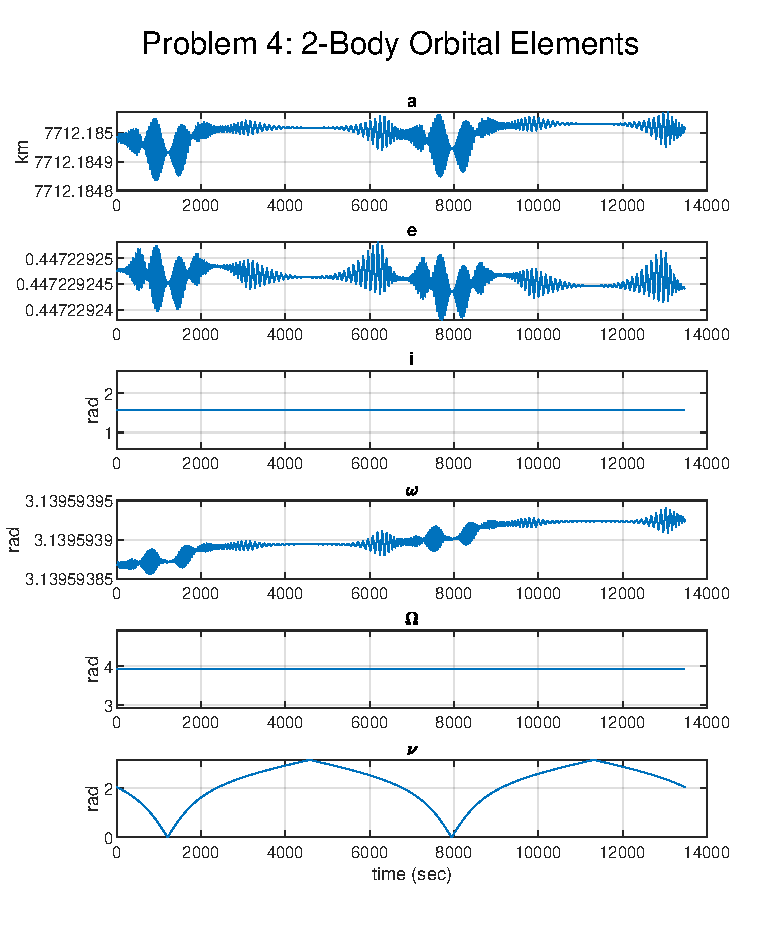
\includegraphics{prob4_2bodoes.pdf}
	\caption{}
	\label{fig:prob4_2bodoes}
\end{figure}

Figure \ref{fig:prob4_angmom} illustrates that the specific angular momentum essentially remains constant throughout the entire orbit. The difference between the maximum and minimum of \textbf{h norm} is 7.204597714007832e-04, which is incredibly small especially when considering that the order of magnitude for all values of \textbf{h norm} is 4. 

\begin{figure}[H]
\centering
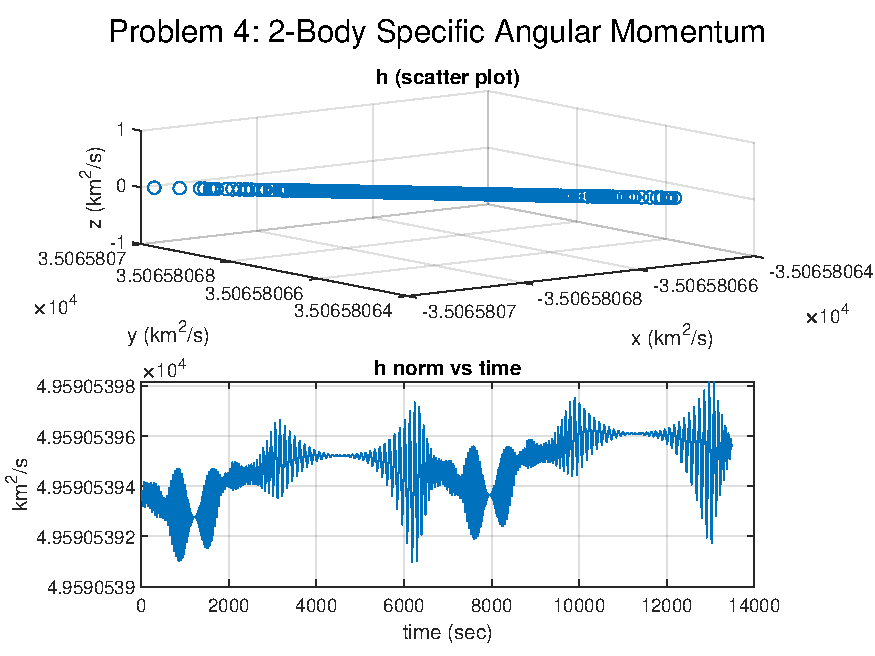
\includegraphics{prob4_angmom.pdf}
\caption{}
\label{fig:prob4_angmom}
\end{figure}

% ================================================================ % 
\section{Problem 5} 

\subsection{Statement} 
\begin{center}
	\fbox{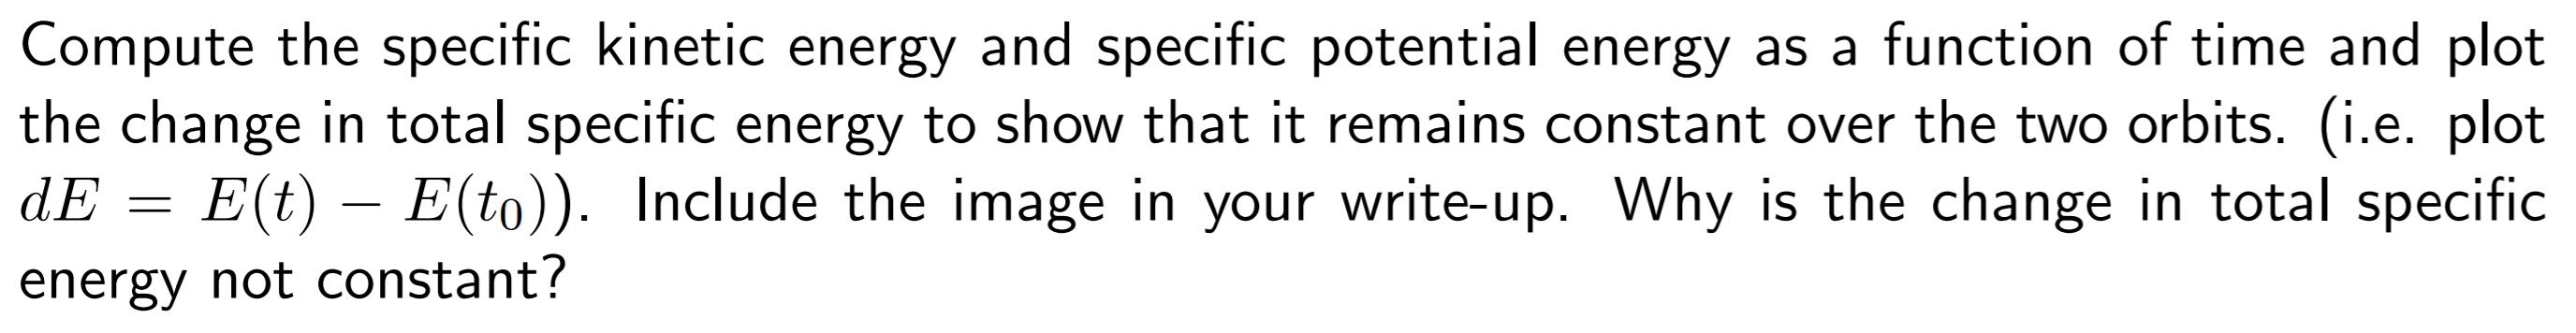
\includegraphics[width=0.9\textwidth]{prob_5.png}} \\
\end{center}

% -------------------------------- % 
\subsection{Solution} 

\begin{figure}[H]
	\centering
	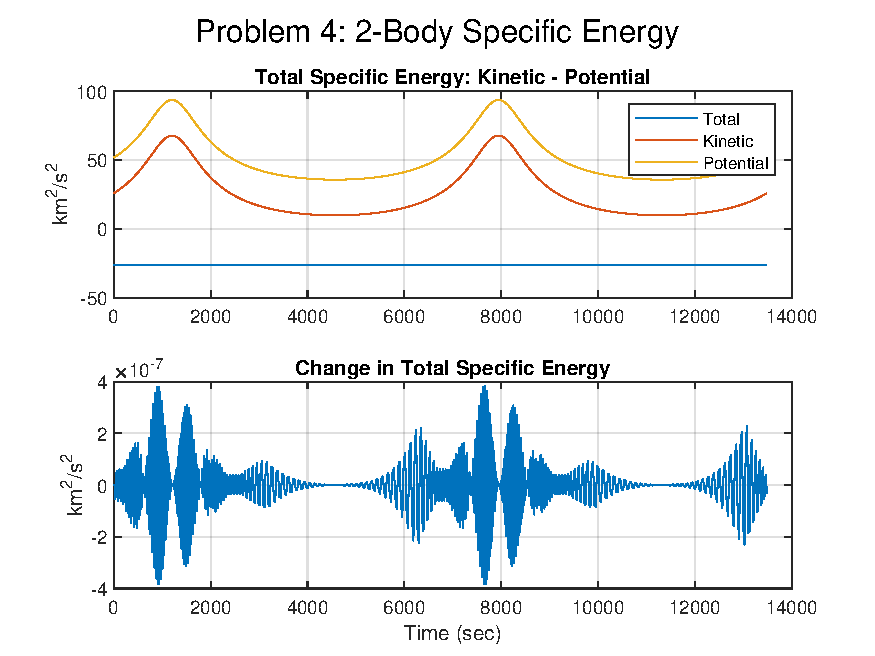
\includegraphics{prob5_energy.pdf}
	\caption{}
	\label{fig:prob5_energy}
\end{figure}

The energy constant of motion is given in Reference \cite{bate_astrodynamics}: 

\begin{equation}
E = \dfrac{v^2}{2} - \dfrac{\mu}{r}
\end{equation}

in which the first term is the "kinetic energy per unit mass," or specific kinetic energy, and the last term is the specific potential energy.  The potential energy will always be negative due to The specific mechanical energy, E, is the sum of the specific kinetic and potential energy and remains constant along its orbit.


%
%% ================================================================ % 
%\section{Problem 2} 
%
%\subsection{Statement} 
%\begin{center}
%\fbox{
\includegraphics[width=0.9\textwidth]{prob_2.png}} \\
%\end{center}
%
%% -------------------------------- % 
%\subsection{Solution} 
%
%An analytical solution provides an exact solution but may not always be easily computed or even possible to obtain, such as in the case of some complex differential equations. Numerical solutions provide approximations which may not exactly match the analytical solution, but can come close within allowable tolerances while being more computationally efficient to obtain. 
%
%The accuracy of the MATLAB ordinary differential equations solver \texttt{ode45} can be adjusted by modifying the options structure through the function \texttt{odeset} \cite{ode45}. RelTol, the relative accuracy tolerance, controls the number of correct digits in the computed answer, and AbsTol, the absolute error tolerance, controls the difference between the computed answer and the true solution \cite{odeset}. Figure \ref{fig:reltol12} shows the error between the numerical and analytical solutions to the displacement of the harmonic oscillator for a relative tolerance of 1e-12, which matches the order of magnitude of the error. When the relative tolerance is adjusted to 1e-6 in Figure \ref{fig:reltol6}, the order of magnitude of the error adjusts accordingly. 
%
%\begin{figure}[H]
%	\centering
%	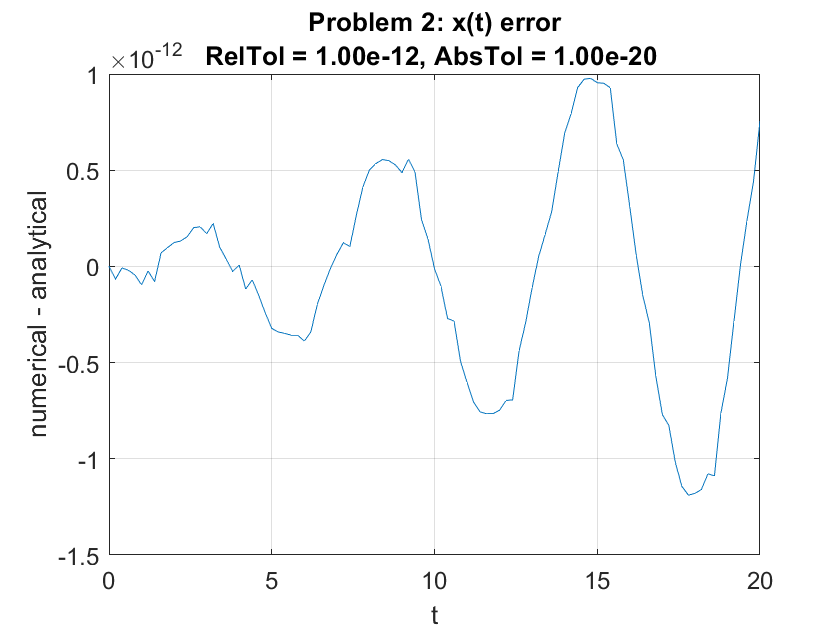
\includegraphics[width=0.7\textwidth]{prob2_err_reltol12.png}
%	\caption{}
%	\label{fig:reltol12}
%\end{figure}
%
%The error grows over time because MATLAB ODE solvers are set up as initial value problems in which the solution at each step is obtained iteratively by propagating the state of the previous step, beginning at the initial conditions \cite{choose_ode}. The truncation of digits and error from numerical integration is propagated as well at each step. 
%
%\begin{figure}[H]
%	\centering
%	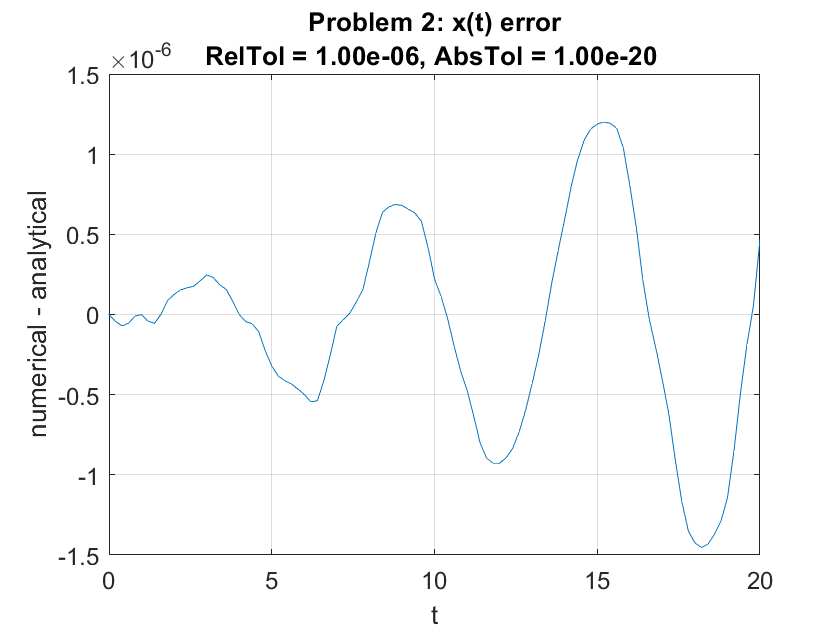
\includegraphics[width=0.7\textwidth]{prob2_err_reltol6.png}
%	\caption{}
%	\label{fig:reltol6}
%\end{figure}
%
%
% ================================================================ % 

\section{Conclusion} 


% ================================================================ % 

\newpage
\section{Appendix} 

HW1 MATLAB code: 

\begin{lstlisting}[basicstyle=\footnotesize]
% ASE 389 Orbit Determination
% HW 0
% Junette Hsin 


%% Problem 1 

t   = linspace( 0, 20, 101 ); 
t   = 0 : 0.2 : 400; 
A   = 1.34; 
phi = pi/3; 
km  = 1; 

x   = A * cos( sqrt( km )*t + phi ); 

name = 'Problem 1: harmonic oscillator x(t)'; 
figure('name', name); 
plot(t, x); 
ylabel('x(t)'); 
xlabel('t'); 
title(name); 
set(gca, 'fontsize', 12); 


%% Problem 2 

y0 = zeros(2,1); 
y0(1) = A * cos(phi); 
y0(2) = - A * sqrt( km ) * sin(phi); 

reltol = 1e-12; 
abstol = 1e-20; 
myoptions   = odeset( 'RelTol', reltol, 'AbsTol', abstol); 
[t, y]      = ode45( @harmoscillator, t, y0, myoptions, km); 

% numerical - analytical 
error = y(:,1)' - x; 

name = 'Problem 2: x(t) error'; 
figure('name', name); 
plot(t, error); 
xlabel('t')
ylabel('numerical - analytical')
title({name ;
sprintf('RelTol = %.2e, AbsTol = %.2e ', reltol, abstol) }); 
set(gca, 'fontsize', 12); 


%% subfunctions 

function dx = harmoscillator( t, x, km )

dx    = zeros(2, 1); 
dx(1) = x(2); 
dx(2) = -km * x(1); 

end 
\end{lstlisting}


% ================================================================ % 
\newpage
\bibliography{sample}

\end{document}
